\subsection{Переменные звёзды}
\term{Переменные звёзды}~--- звёзды, у которых наблюдаются колебания блеска.   Для отнесения звезды к разряду переменных достаточно, чтобы блеск звезды хотя бы однажды претерпел изменение.

Переменные звёзды делятся на две большие группы: \imp{затменные} и \imp{физические}, причём физические подразделяются на \imp{пульсирующие} и \imp{эруптивные}.

\begin{wrapfigure}[11]{l}{0.47\tw}
    \centering
    \vspace{-1.2pc}
    \tikzsetnextfilename{light-curve-d-cep}
    \begin{tikzpicture}
        \begin{axis}[
            height    =    4.5cm,
            width    =    .5\tw,
            xlabel    =    {Фаза},
            ylabel    =    {Блеск $m$, $~^m$},
            ymax    =    8.,
            ymin    =    6.5,
            y dir    =    reverse,
            xmax    =    1,
            xmin    =    0
        ]
            \addplot+[only marks, mark = o, mark options={scale=0.2, black}] table[x=f, y=m]{data/light-curve-D-Cep.txt};
        \end{axis}
    \end{tikzpicture}
    \caption{Кривая блеска переменной типа $\delta$\,Cep}
    \label{pic:d-cep}
\end{wrapfigure}
К \term{пульсирующим} переменным  относят те звёзды, переменность которых вызвана процессами, происходящими в их недрах. Эти процессы приводят к периодическому изменению температуры поверхности и радиуса фотосферы, а вместе с тем и блеска звезды. Период переменности варьируется в пределе от долей суток до~нескольких~лет в зависимости от типа переменной.

Классический пример пульсирующих переменных звёзд~--- \imp{цефеиды}, названные в честь первой открытой переменной данного типа~--- $\delta$\,Cep. Абсолютную звёздную величину $M$ и период $T$ (в сутках) цефеид связывает соотношение
\begin{equation}
    M = -1.43^m - 2.81\lg T.
\end{equation}

\begin{wrapfigure}[11]{r}{0.47\tw}
    \centering
    \vspace{-1.2pc}
    \tikzsetnextfilename{light-curve-rr-lyr}
    \begin{tikzpicture}
        \begin{axis}[
            height    =    4.5cm,
            width    =    .5\tw,
            xlabel    =    {Фаза},
            ylabel    =    {Блеск $m$, $~^m$},
            ymax    =    12.5,
            ymin    =    11.5,
            y dir    =    reverse,
            xmax    =    1,
            xmin    =    0
        ]
            \addplot+[only marks, mark = o, mark options={scale=0.2, black}] table[x=f, y=m]{data/rr-lyr.txt};
        \end{axis}
    \end{tikzpicture}
    \caption{Кривая блеска переменной типа RR~Lyr} % http://www.astrouw.edu.pl/asas/?psect=acvs&page=details&id=000405-1659.8
    \label{pic:light-curve-rr-lyr}
\end{wrapfigure}
Ещё один класс пульсирующих переменных звёзд~--- \imp{переменные типа RR~Lyr}, прототипом которого стала звезда RR~Lyr. Такие звёзды довольно стары и маломассивны. Они являются гигантами спектрального класса А, лежащими на горизонтальной ветви диаграммы Герцшпрунга\,--\,Рассела. Светимости этих звёзд различаются слабо и составляют порядка $40L_\odot$. Поэтому они, как и цефеиды, используются в качестве стандартных свеч.

К \term{эруптивным} переменным звёздам относятся звёзды, меняющие свой блеск нерегулярно или единожды за время наблюдений. Все изменения блеска эруптивных звёзд связывают с бурными процессами и вспышками в их хромосферах и коронах. К таким, например, относятся \imp{новые} и \imp{сверхновые}.

\term{Затменно-переменные} звёзды --- системы из двух звёзд, суммарный блеск которых периодически изменяется с течением времени. Причиной изменения блеска могут быть затмения звёзд друг другом, или изменение их формы взаимной гравитацией в тесных системах. На \picRef{pic:w-uma}\,--\,\ref{pic:b-lyr}  представлены кривые блеска затменно-переменных звёзд трёх основных типов.

\begin{figure}[!h]
    \centering
    \begin{minipage}[c]{0.49\tw}
        \tikzsetnextfilename{light-curve-w-uma}
        \begin{tikzpicture}
            \begin{axis}[
                height    =    4.5cm,
                width    =    \tw,
                xlabel    =    {Фаза},
                ylabel    =    {Блеск $m$, $~^m$},
                ymax    =    1.1,
                ymin    =    -.1,
                y dir    =    reverse,
                xmax    =    1,
                xmin    =    0
                ]

                \addplot[smooth] table[x=t, y=m]{data/light-curve-W-UMa.txt};
            \end{axis}
        \end{tikzpicture}
    \end{minipage}
    \hfill
    \begin{minipage}[c]{0.49\tw}
        \centering
        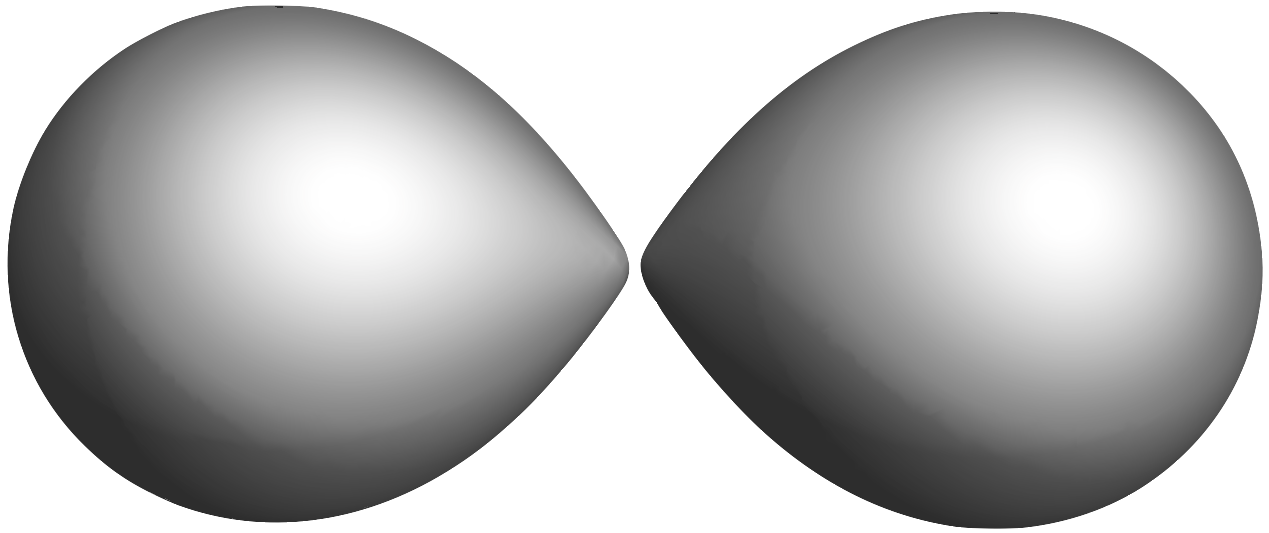
\includegraphics[width = .9\tw]{w-uma}
    \end{minipage}
    \caption{Кривая блеска переменной типа W\,UMa}
    \label{pic:w-uma}
\end{figure}

\begin{figure}[!h]
    \centering
    \begin{minipage}[c]{0.49\tw}
        \tikzsetnextfilename{light-curve-b-per}
        \begin{tikzpicture}
            \begin{axis}[
                height    =    4.5cm,
                width    =    \tw,
                xlabel    =    {Фаза},
                ylabel    =    {Блеск $m$, $~^m$},
                ymax    =    .7,
                ymin    =    -.1,
                y dir    =    reverse,
                xmax    =    1.,
                xmin    =    .0
                ]
                \addplot[smooth] table[x=t, y=m]{data/light-curve-B-Per.txt};
            \end{axis}
        \end{tikzpicture}
    \end{minipage}
    \hfill
    \begin{minipage}[c]{0.49\tw}
        \centering
        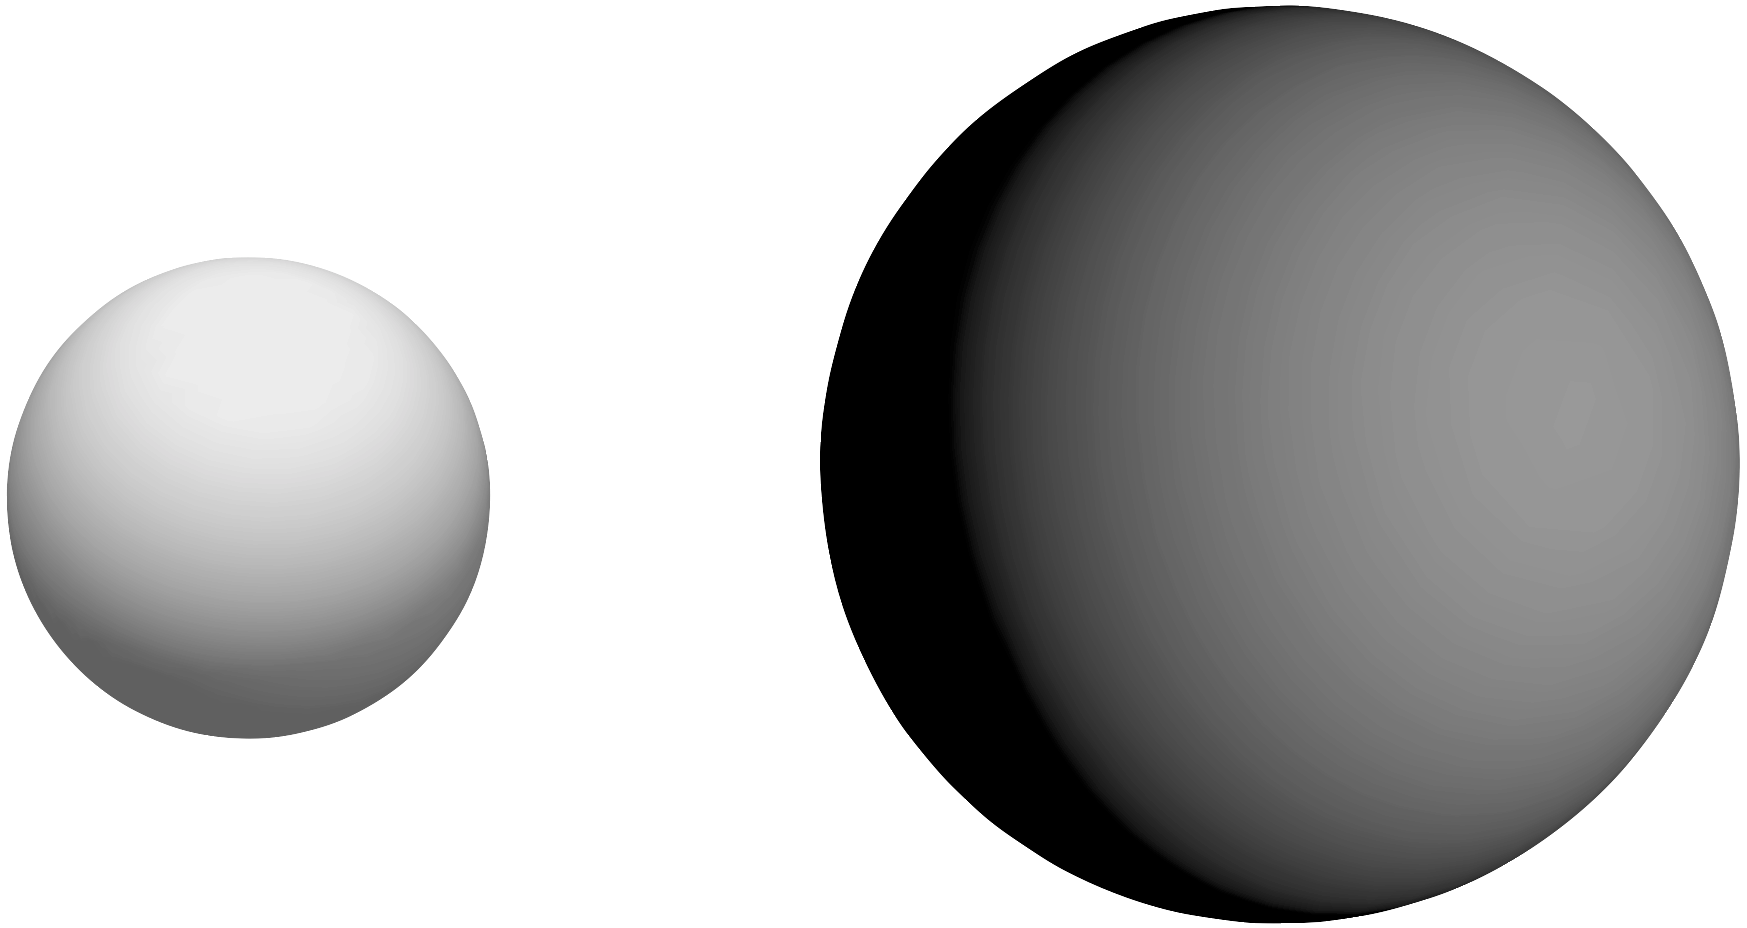
\includegraphics[width=.9\tw]{b-per}
    \end{minipage}
    \caption{Кривая блеска переменной типа $\beta$\,Per}
\end{figure}
